\documentclass{article}
\usepackage{graphicx} % new way of doing eps files
\usepackage{listings} % nice code layout
\usepackage[usenames]{color} % color
\definecolor{listinggray}{gray}{0.9}
\definecolor{graphgray}{gray}{0.7}
\definecolor{ans}{rgb}{1,0,0}
\definecolor{blue}{rgb}{0,0,1}
% \Verilog{title}{label}{file}
\newcommand{\Verilog}[3]{
  \lstset{language=Verilog}
  \lstset{backgroundcolor=\color{listinggray},rulecolor=\color{blue}}
  \lstset{linewidth=\textwidth}
  \lstset{commentstyle=\textit, stringstyle=\upshape,showspaces=false}
  \lstset{frame=tb}
  \lstinputlisting[caption={#1},label={#2}]{#3}
}


\author{Josh Young}
\title{Lab 11}

\begin{document}
\maketitle

\section{Introduction}
In Lab 11, the user was tasked with completing the Write Back stage as well as construct the full pipeline. Writeback is the last stage for the pipeline, and uses outputs from memory and the ALU. The pipeline consists of 5 stages, which are Fetch, Decode, Execute, Memory, and Write Back. With these 5 stages, the user was able to simulate a full MIPS machine to a degree, however there are limits to the pipeline as it currently is, namely, one must run several 'no-ops' between instructions because the current pipeline doesn't include a forwarding unit. The pipeline was simulated using verilog code via Vivado.

\section{Interface}
As stated before, there are 5 stages to the MIPS machine pipeline. However, all inputs and outputs are self contained with the exception of a 'run' input, which serves as the only exterior input. Run acts as a booting process for the pipeline and only consists of 1 wire. The Writeback stage is on the simple side, since a single multiplexer builds it. There are 2 inputs, a control and an output. The inputs come from the result of the ALU, and from memory.  The control wire comes from the register file, and the output, 'result', is fed into the 'write data' input for the register file.  

\section{Design}
The pipeline begins with the Fetch stage. This consists of a multiplexer and an adder to come up with program counts in order to fetch instructions from memory. Once the instruction has been fetched, the signal reaches the second part of the pipeline, the Decode stage. Here, the instruction's bits are grouped and distributed across a sign extender, and register file to in order to get values from the registers. After that, the signals reach the Execute stage which encompasses more multiplexers, and an ALU. After the ALU calculates a result, the result as well as other signals reaches the next stage in the pipeline, the Memory stage. Here is were the system finds out where to branch, as well as read and write. After the Memory stage, the pipeline finally reaches the last stage which is the Writeback stage. This is were the last of the signals loop back to the fetch and decode stage.

\section{Implementation}
The code used for constructing the pipeline can be seen in Listing~\ref{code:pipeline} on page~\pageref{code:pipeline}.

\Verilog{Verilog code for constructing the pipeline.}{code:pipeline}{../code/pipeline.v}

\section{Test Bench Design}
The lab required implementation of a testbench for the pipeline, but in this case, everything was self contained so the testbench is the same as the pipeline code.

\section{Simulation}
The timing diagram shows that the pipeline is able to augment the program count and run autonomously based off of the instructions given in instruction memory. Note that the ALU result shows the appropriate answer based off of the inputs, and the read data from memory shows high impedance when read data is low. The timing diagram for the pipeline can be viewed in Figure~\ref{fig:test}. 
\section{Conclusions}
The goal for this lab was to create the Writeback stage, implement the entire pipeline for MIPS, and run with test files. The timing diagram shows that the behavior for the pipeline was as expected. However, there is a possibility that the current edition of this pipeline could run into data hazards. This is due to the lack of a forwarding unit which supplies decode, execute, and memory with the appropriate data so that no data hazard occurs.
\begin{figure}
	\begin{center}
		\caption{Timing diagram for the pipeline test.}\label{fig:test}
		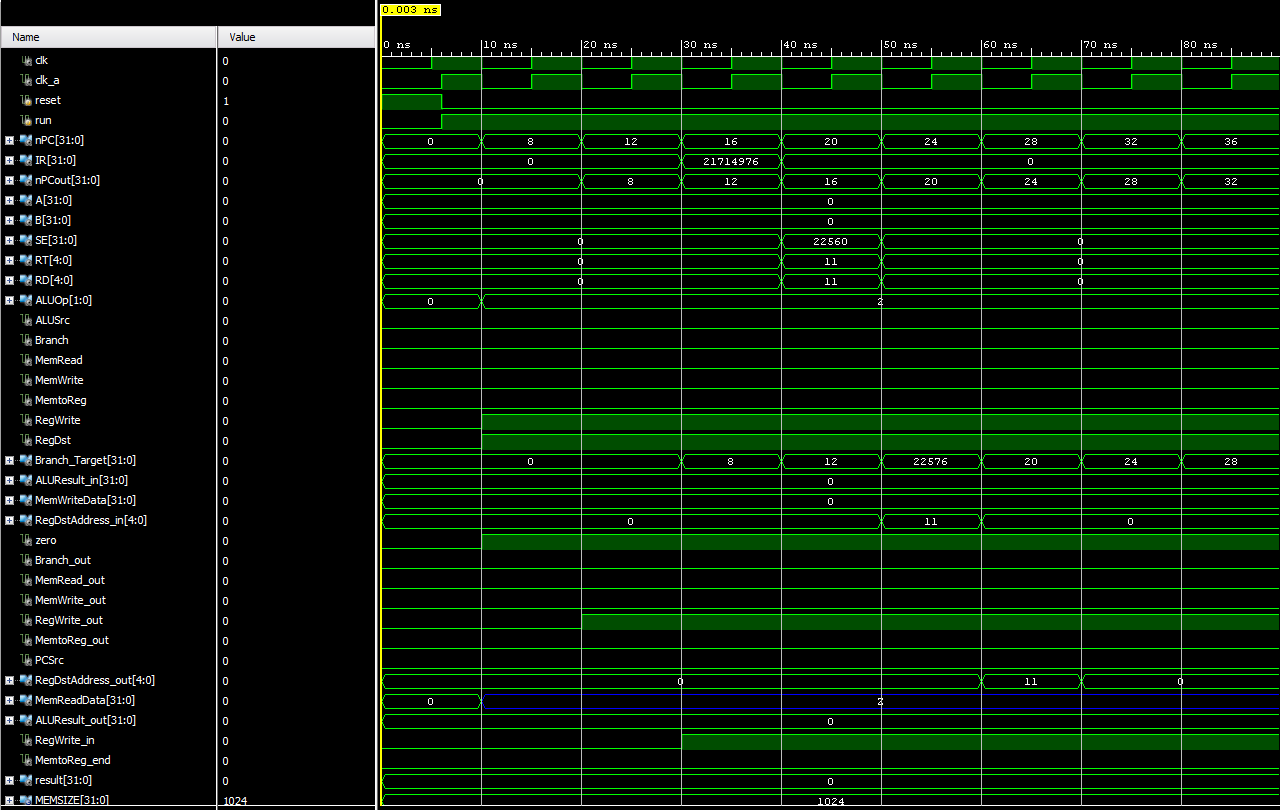
\includegraphics[width=0.9\textwidth]{../images/PIPELINEPIC.png}
	\end{center}
\end{figure}

\end{document} 